\documentclass{beamer}

\usepackage[utf8]{inputenc} % Ensure proper encoding
\usepackage{graphicx} % For including images
\usepackage{hyperref} % For hyperlinks
\usepackage{amsmath,amsfonts,amssymb} % For mathematical symbols and equations
\begin{document}

\title{The State Capacity Ceiling on Tax Rates: Evidence from Randomized Tax Abatements in the DRC}
\author{Augustin Bergeron, Gabriel Z. Tourek \& Jonathan L. Weigel}
\date{\today}

\frame{\titlepage}


\begin{frame}
\frametitle{Introduction}
\begin{itemize}
\item We discussed in an earlier class that tax enforcement is crucial. You just not only need to detect but also recover evasion. 
\item However, changes in tax enforcement effectively increase effective tax rates as reporting increases. Therefore, there can be a trade off between tax enforcement vs tax rates.
\item If you need to raise R new dollars, either increase enforcement or increase tax rates
\item In Jensen paper we discussed that imperfect enforcement through informality can be redistributive, therefore it might be sometimes better to increase taxes rather than enforcement.
\end{itemize}
\end{frame}

\begin{frame}
\frametitle{This paper}
\begin{itemize}
    \item How tax enforcement and tax rates jointly effect fiscal capacity in low income countries? 
    \item Tax compliance is low:  on average, 8.8\% of property owners paid the property tax in 2018.
    \item Randomly assign 38,028 property owners to the status quo tax rate or to a rate reduction.
    \item Changes in reported tax liabilities indicate that current rate was above revenue maximizing threshold. 
    \item Then, through randomized enforcement
letters and random assignment of tax collectors shows that the RMTR increases with enforcement. 
\item Tax rates and enforcement are thus complementary levers. 
  
\end{itemize}
\end{frame}

\begin{frame}{Experiment}
\begin{itemize}
    \item Exploit random variation in the joint distribution of tax
rates and tax enforcement in the DRC, a very low capacity state and one of the world’s
poorest countries.
    \item In its 2018 property tax
campaign, the Provincial Government of Kasaï-Central randomly assigned tax abatements
at the property level. 
\item The 38,028
properties in the city were randomly assigned to the status quo annual tax liability (control)
or a reduction of 17\%, 33\%, or 50\%.
\item Taxpayers were just informed about their liability. 
\item Use this variation to estimate the elasticity of tax compliance
and revenue with respect to the tax rate as well as the RMTR. 
\item Randomized enforcement messages on
tax notices and random assignment of tax collectors to neighborhoods to study how the
RMTR responds to changes in the enforcement environment.
\end{itemize}
\end{frame}

\begin{frame}{Results: Does lower tax rates increase compliance?}
\begin{figure}
    \centering
    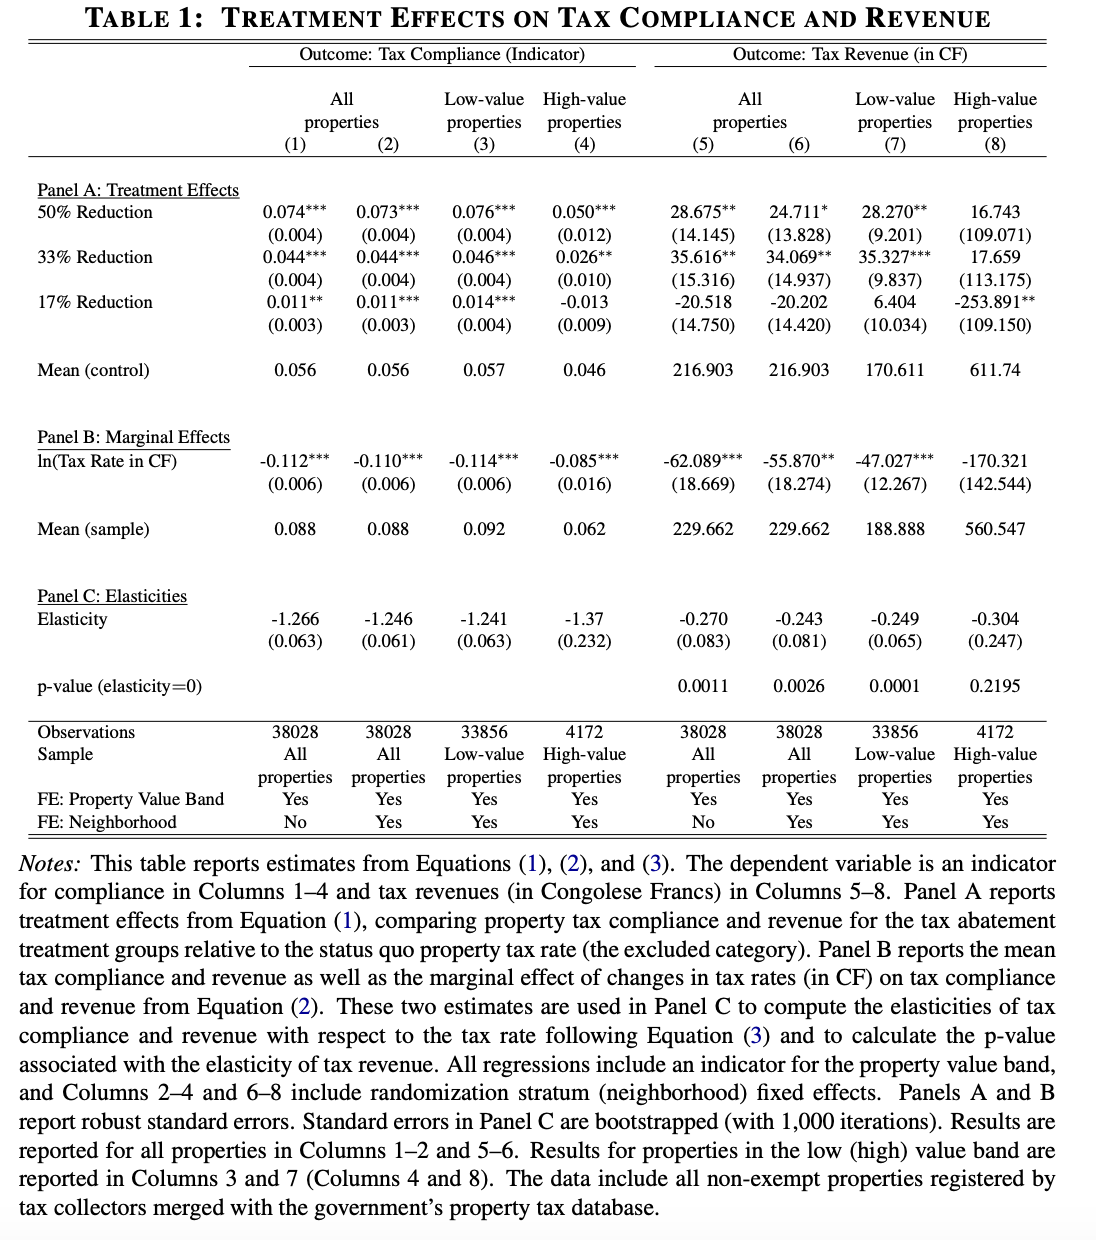
\includegraphics[height=\textheight,width=\textwidth]{Paper Presentations/The State Capacity Ceiling on Tax Rates/T1.png}
    \label{fig:enter-label}
\end{figure}
\end{frame}

\begin{frame}{Mechansims}
\begin{figure}
    \centering
    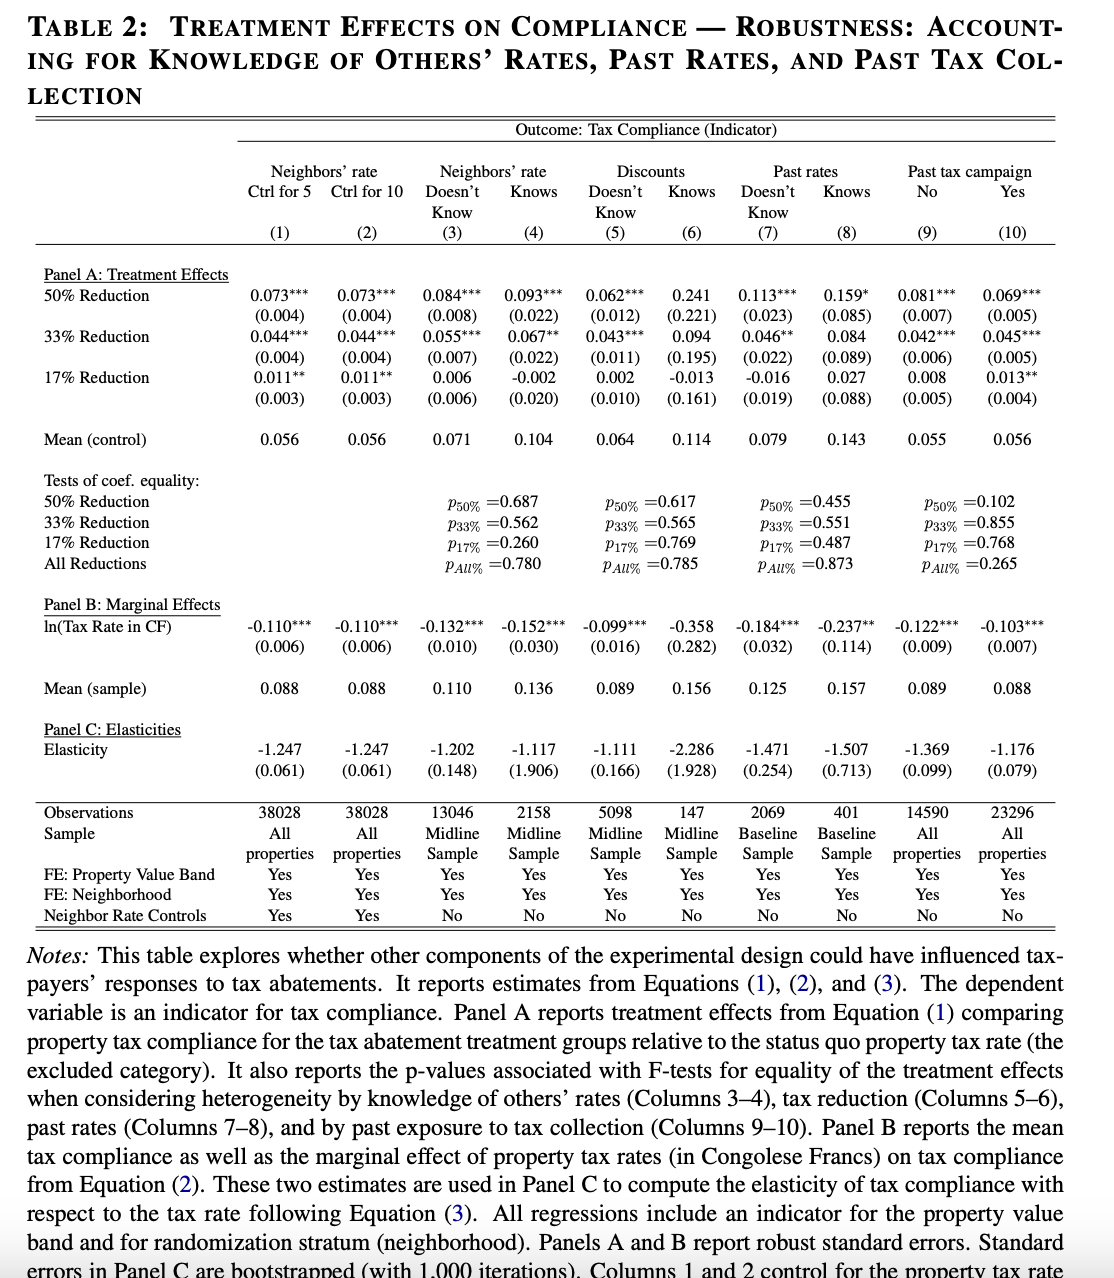
\includegraphics[height=\textheight,width=\textwidth]{Paper Presentations/The State Capacity Ceiling on Tax Rates/T2.png}
    \label{fig:enter-label}
\end{figure}
\end{frame}

\begin{frame}{RMTR}
\begin{figure}
    \centering
    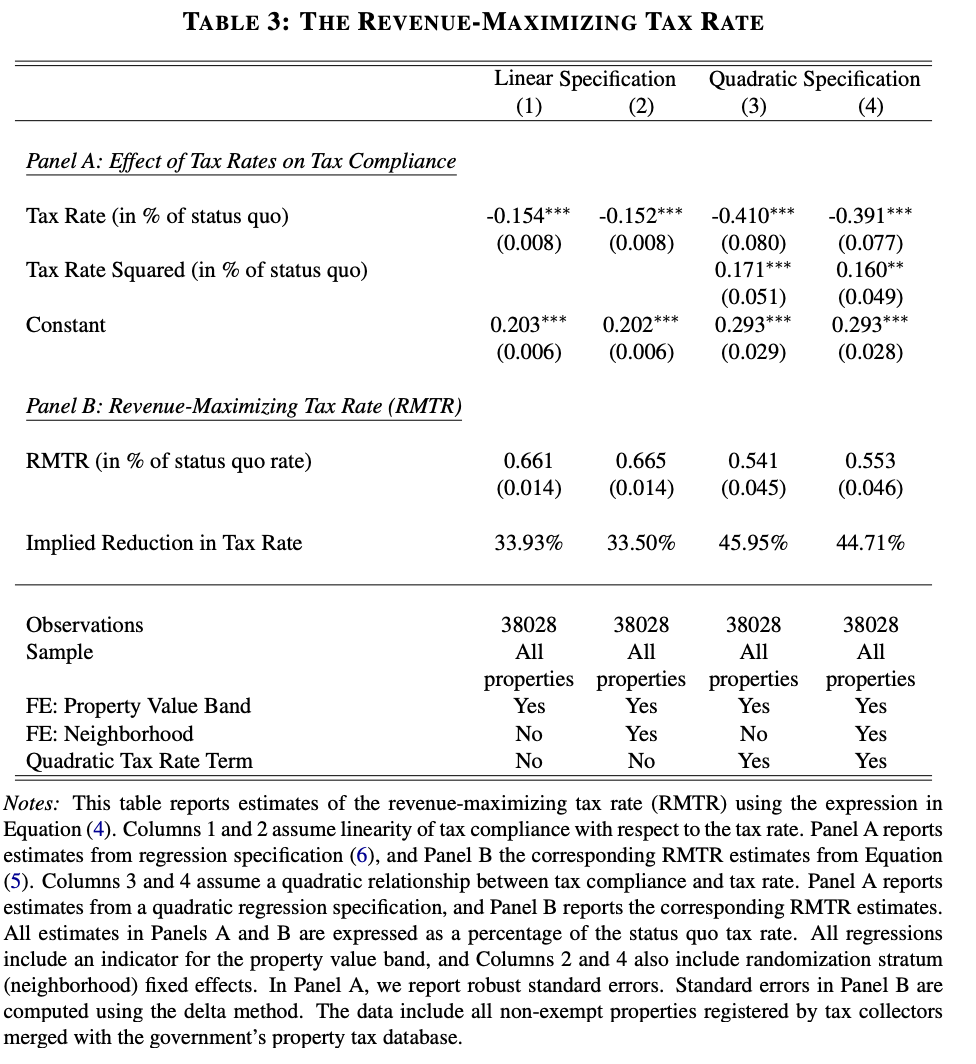
\includegraphics[width=\textwidth,height=0.8\textheight]{Paper Presentations/The State Capacity Ceiling on Tax Rates/T3.png}
    \label{fig:enter-label}
\end{figure}
\end{frame}

\begin{frame}{RMTR and Enforcement}
\begin{figure}
    \centering
    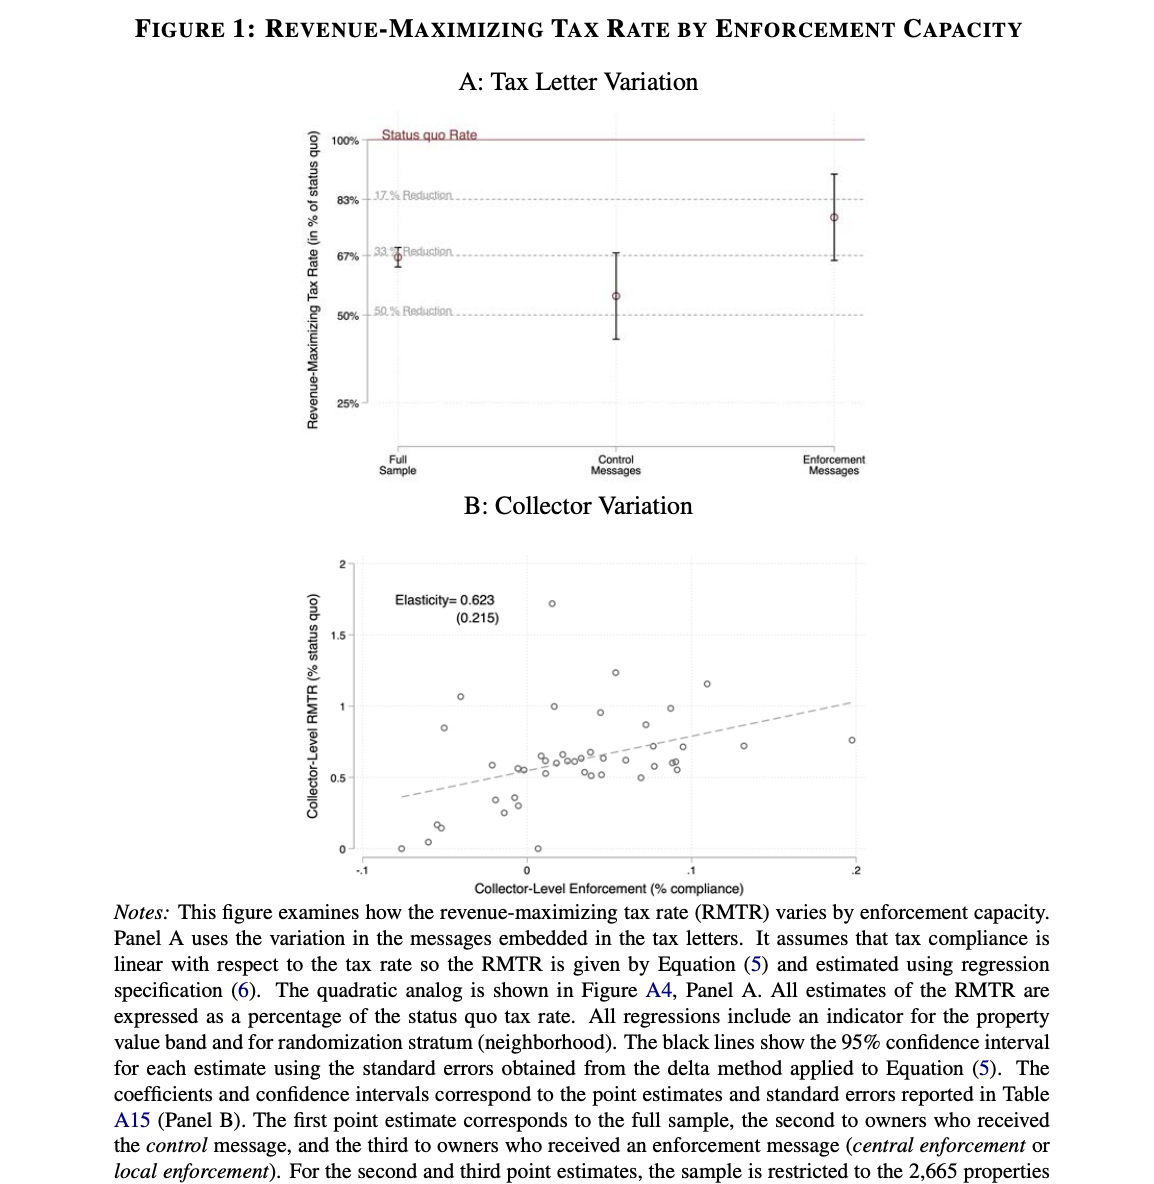
\includegraphics[height=\textheight,width=\textwidth]{Paper Presentations/The State Capacity Ceiling on Tax Rates/F1.png}
    \label{fig:enter-label}
\end{figure}
\end{frame}



\begin{frame}
\frametitle{Rates and Enforcement as Complements}
\begin{figure}
    \centering
    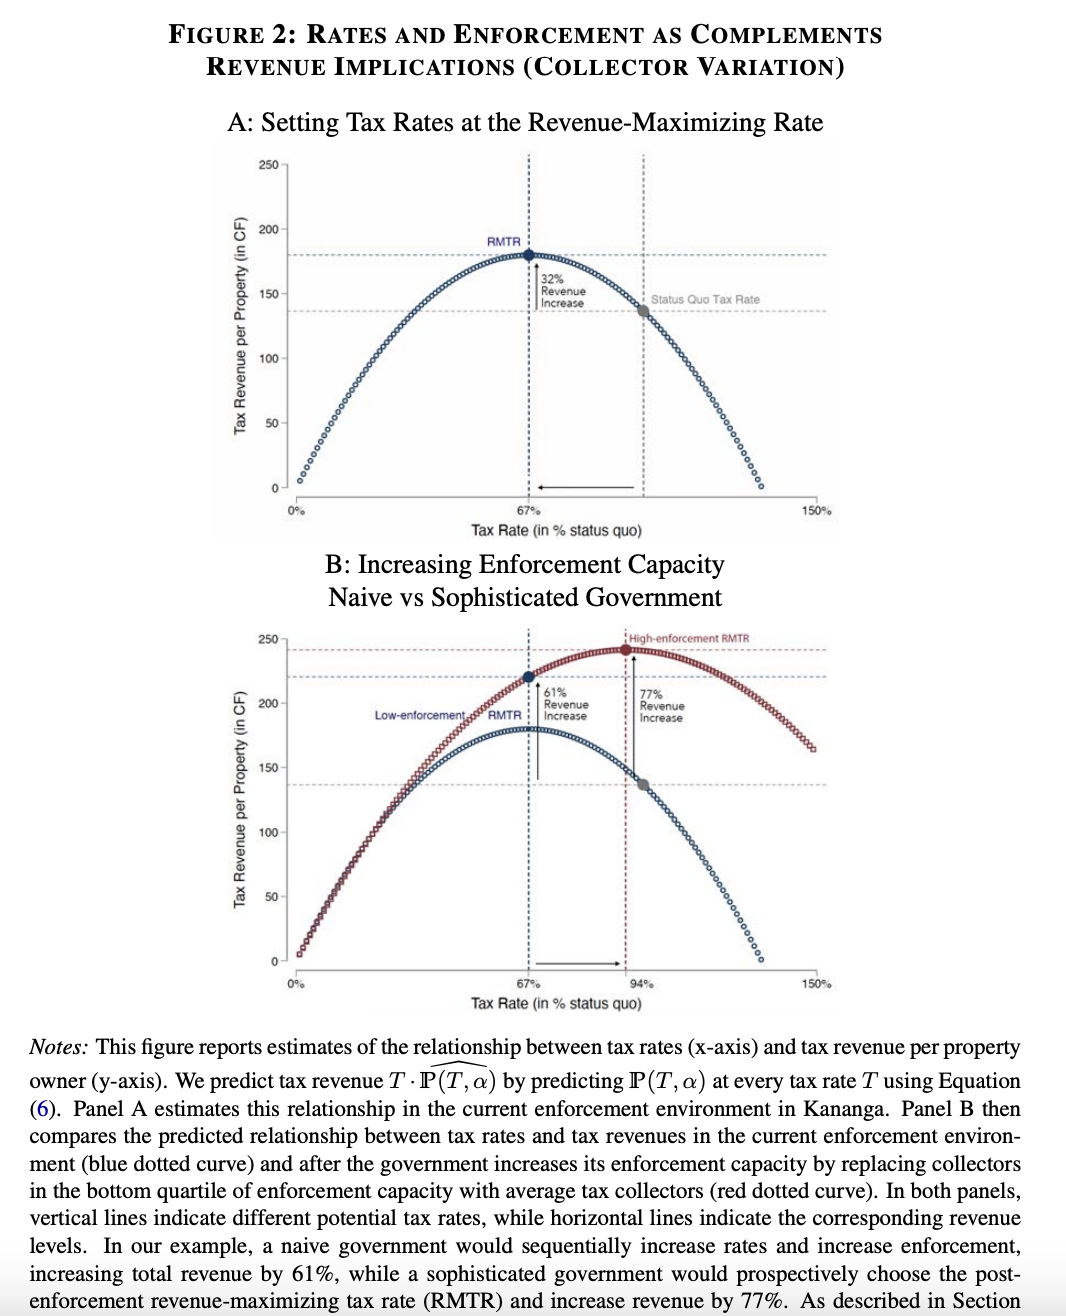
\includegraphics[height=0.9\textheight,width=\textwidth]{Paper Presentations/The State Capacity Ceiling on Tax Rates/F2.png}
\end{figure}
\end{frame}

\begin{frame}{Questions}
    \begin{itemize}
        \item Does it mean that when tax rate is lower, it is not optimal for taxpayers to evade it and therefore they pay it?
        \item Does it mean governments with weak state capacity should start with very low tax rates?
        \item What does this mean for other taxes, in particular taxation of businesses?
        \item It is very important to think about this question in public finance that when govt has very low capacity and they want to start raising revenue to build the capacity, what are lessons there?
    \end{itemize}
\end{frame}
\begin{frame}
\frametitle{Conclusions}
\begin{itemize}
\item Tax rates and enforcement are thus complementary levers. 
\item Jointly optimizing tax rates and
enforcement would lead to 26\% higher revenue gains than optimizing them independently.
\item These
findings provide experimental evidence that low government enforcement capacity sets a binding
ceiling on the revenue-maximizing tax rate in some developing countries, thereby demonstrating
the value of increasing tax rates in tandem with enforcement to expand fiscal capacity
\end{itemize}
\end{frame}

\end{document}

\begin{frame}
  \titlepage
\end{frame}



\end{document}
